\chapter{Оптимизации в векторном компиляторе}\label{ch:lowering}

\section{Метод ступенчатого понижения}\label{sec:lowering/passes}

Метод ступенчатого понижения заключается в чередовании понижения уровня промежуточного представления с оптимизациями, допускаемыми текущим уровнем без изменения промежуточного представления. Пусть у вас есть некий IR высокого уровня (например LLVM IR) со сложэными высокуровневыми конструкциями в нём. Центральным наблюдением метода является возможность исключить ряд этих констуркций (например заменить операции с памятью на низкоуровневые операции целевой архитектуры) но при этом сохранить данный IR высокого уровня прежним и до момента понижения дать на очередной ступеньке отработать всем стандартным оптимизациям которые требуют обобщённого представления памяти (например объединяющим загрузки в соседние места памяти).

Место ступенчатого понижения в списке трансформаций графического компилятора выбирается из следующих соображений.

\begin{enumerate}
\item Должна отработать трансляция из SPIRV.
\item Также должны отработать основные высокоуровневые платформенно-независимые оптимизации.
\item При этом не должны быть легализованы инструкции и не должна быть начата кодогенерация.
\end{enumerate}

\begin{figure}[ht]
    \centerfloat{
        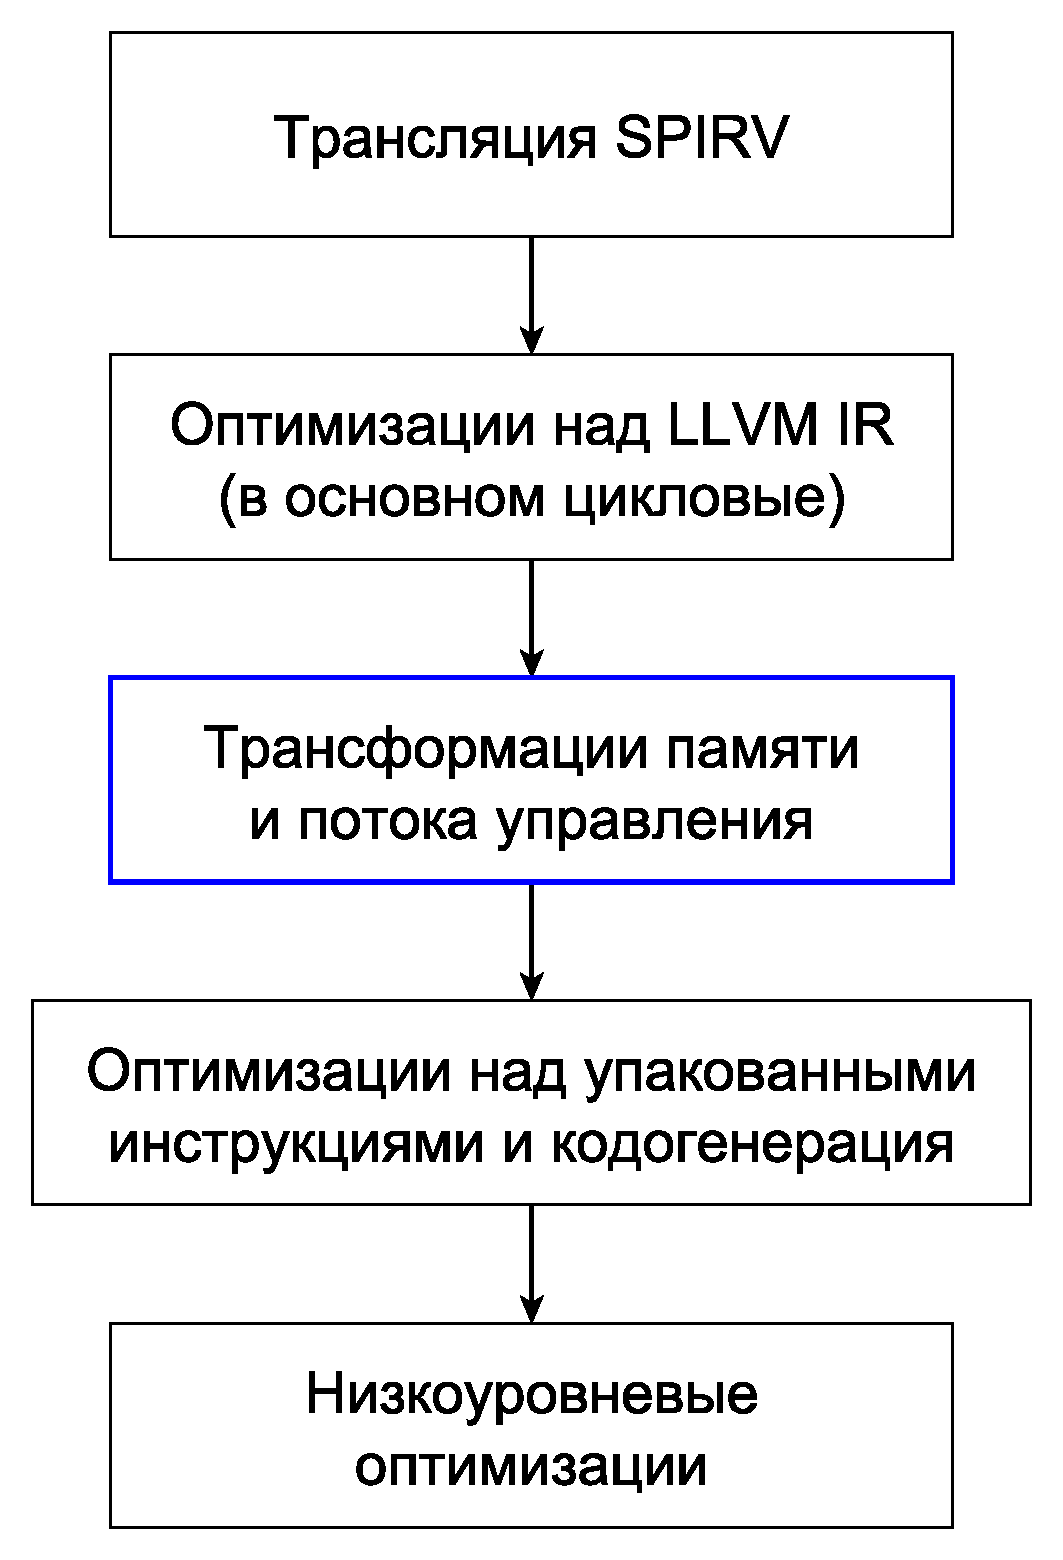
\includegraphics[scale=0.6]{Vladimirov/images/highlevel-mgr.pdf}
    }
    \caption{Высокоуровневый список трансформаций}\label{fig:highlevel-mgr}
\end{figure}

Высокоуровневая схема менеджера пассов представлена на рисунке~\cref{fig:highlevel-mgr}. Выбор места обосновывается как результатами экспериментов, так и следующими соображениями.

\begin{itemize}
\item Трансформация операций копирования возможна только после того как эта операция распознана как идиома, то есть после оптимизаций над высокоуровневым IR.
\item Разрешение адресных пространств может породить много платформенно-зависимого кода и должно идти до оптимизаций над легализованными инструкциями.
\item Трансформация приватных операций с памятью и выделение спиллов должно идти после цикловых оптимизаций, но до вставки пролога и эпилога.
\item TODO: расписать все соображения.
\end{itemize}

Важно подчеркнуть, что метод применим к любой системе и любому уровню промежуточного представления с минимальными модификациями. 

\begin{figure}[ht]
    \centerfloat{
        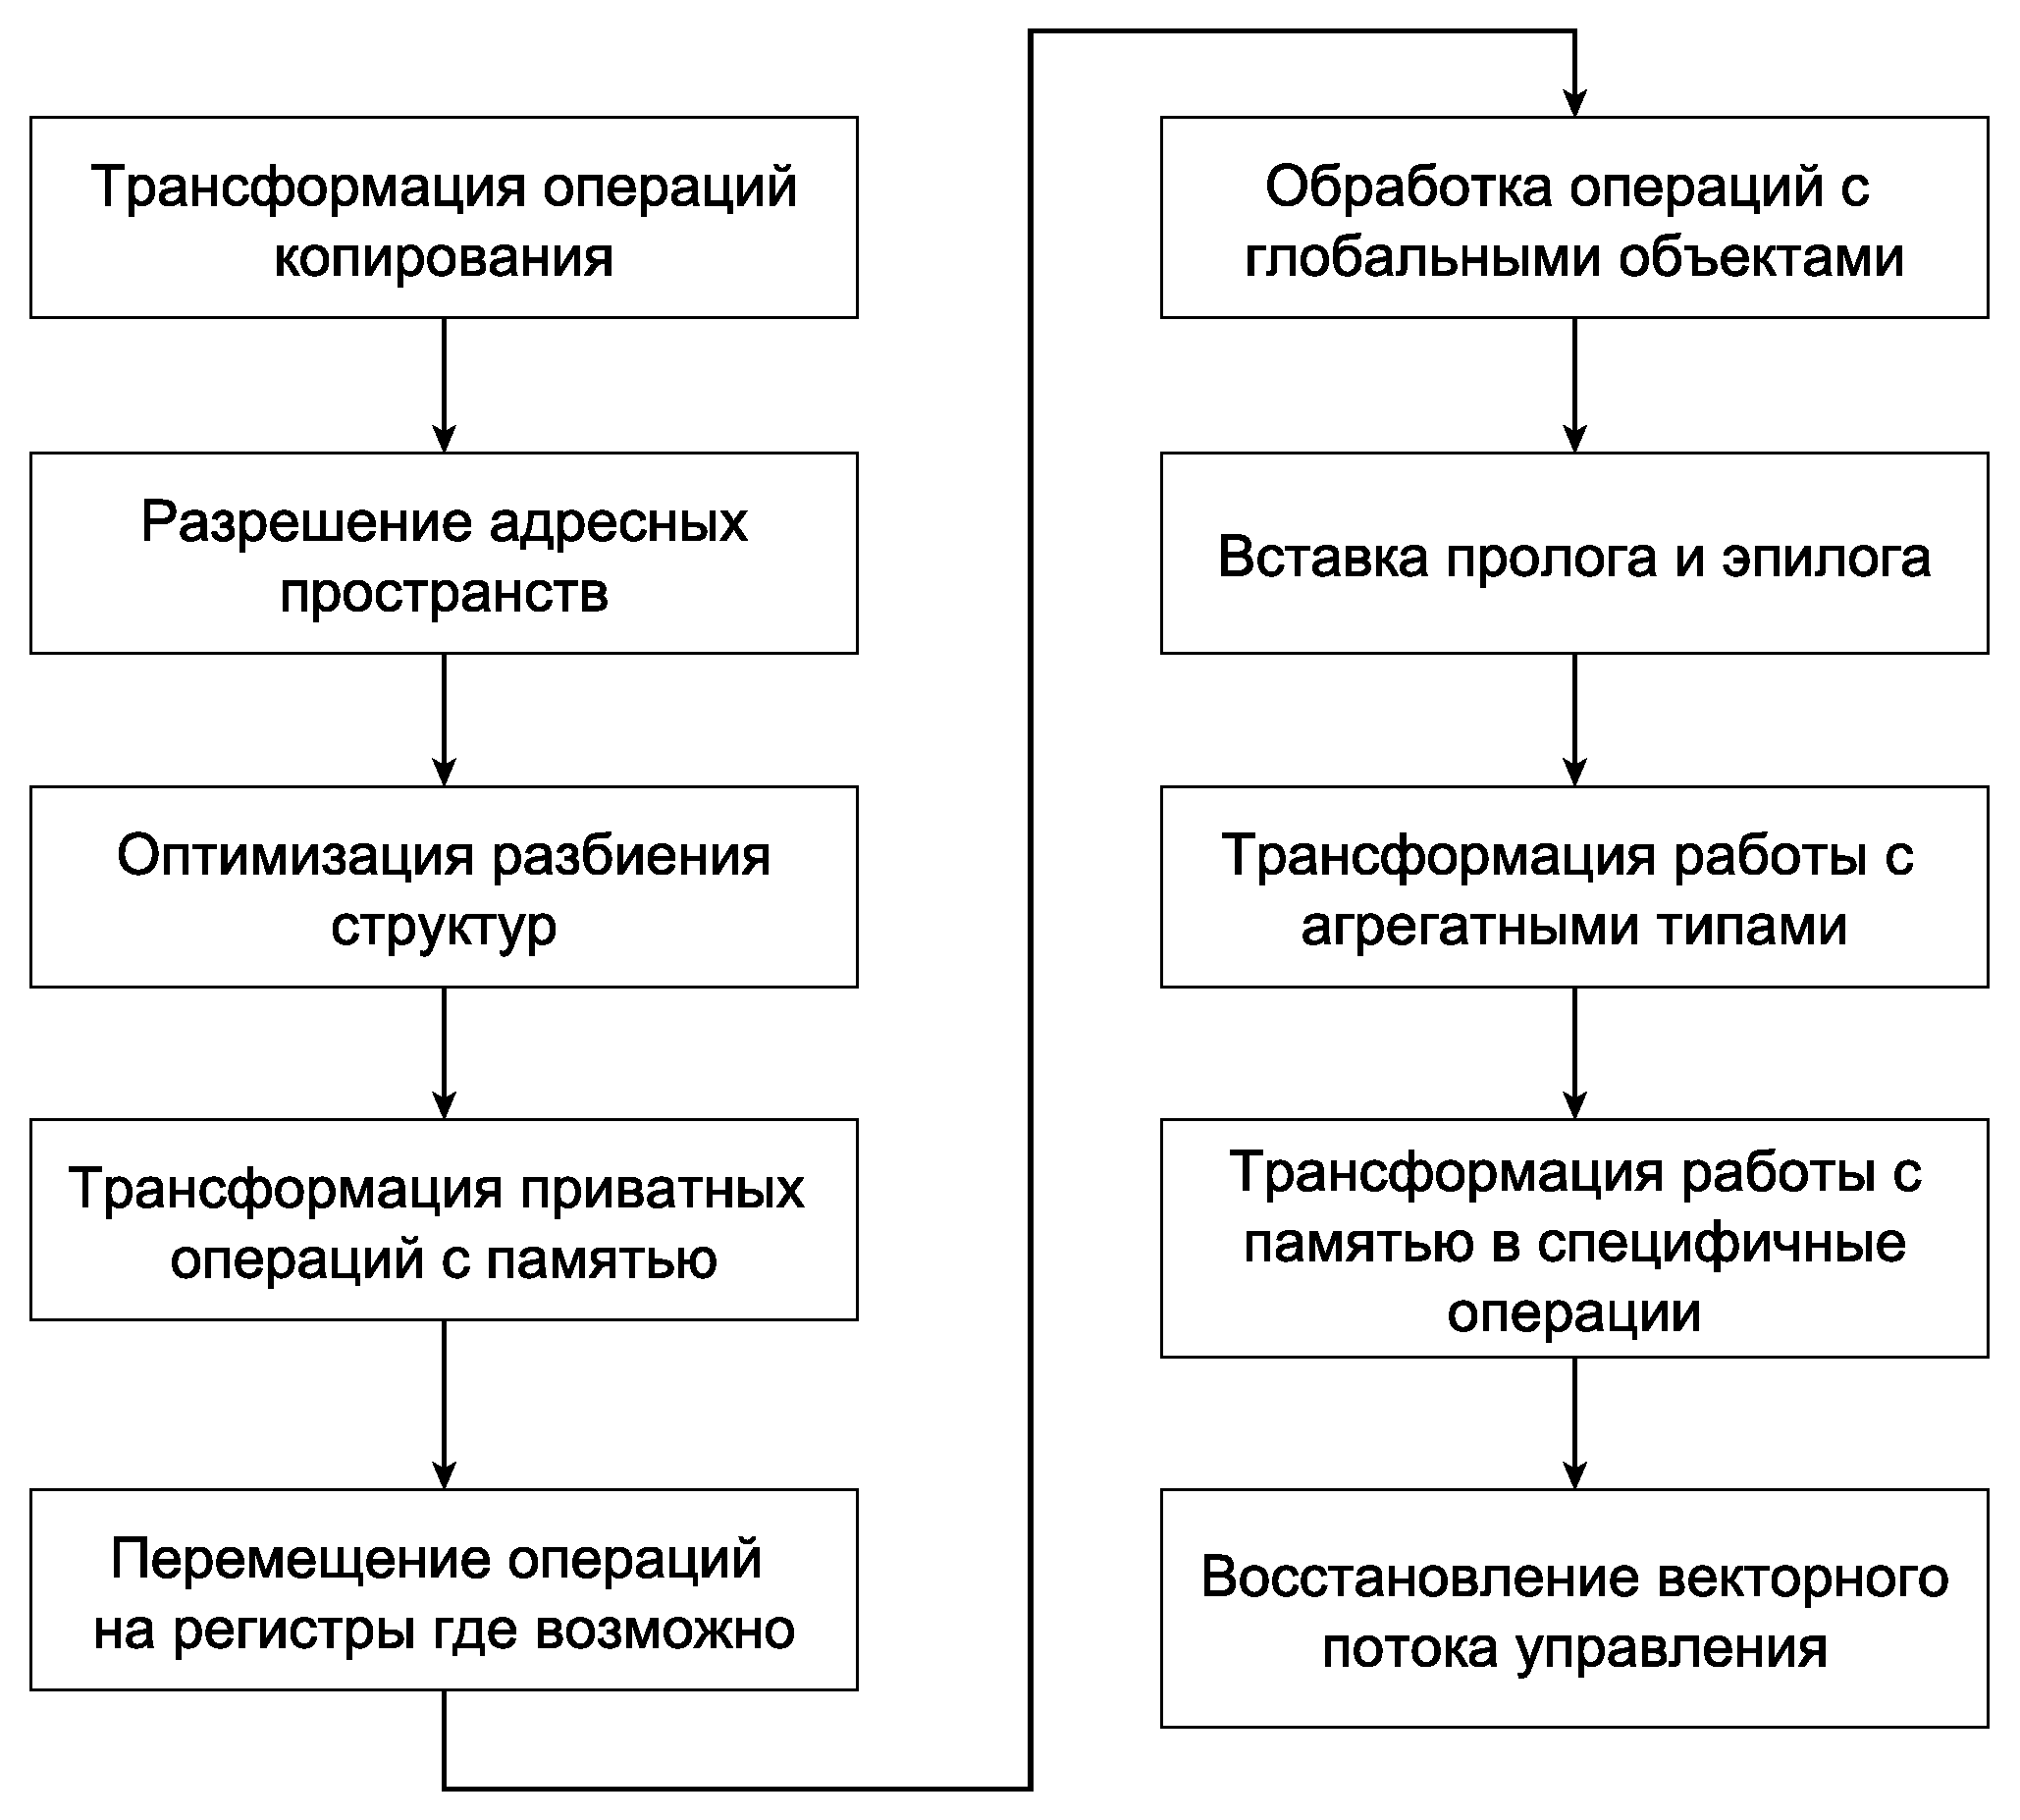
\includegraphics[scale=0.4]{Vladimirov/images/passmgr.pdf}
    }
    \caption{Детальный список трансформаций}\label{fig:passmgr}
\end{figure}

Детальный список трансформаций представлен на рисунке~\cref{fig:passmgr}. В нём есть два вида трансформаций -- обязательные легализации необходимые для представления высокоуровневых конструкций для векторной системы команд и необязательные оптимизации, которые оптимизируют представление, делая его более подходящим для высокоэффективных вычислений.

\subsection{Высокоуровневое представление}\label{subsec:lowering/passes/highlevel}

Представление на IR высокого уровня (HIR, high-level IR) после высокоуровневого языка содержит адресные пространства и трансформации типов указателей между типами пространств адресов. Кроме того там используются обобщённые операции загрузки и сохранения.

\begin{ListingEnv}[!h]
    \captiondelim{ }
    \caption{Пример представления на HIR}\label{lst:lowering/irrep}
    \begin{lstlisting}[language=llvm]
%4 = tail call i32 @llvm.genx.group.id.x()
%5 = extractelement <3 x i32> %local.size, i32 0
%6 = mul i32 %4, %5
%7 = extractelement <3 x i32> %local.id, i32 0
%8 = add i32 %6, %7
    \end{lstlisting}
\end{ListingEnv}

Листинг~\cref{lst:lowering/irrep} показывет загрузку вектора группового идентификатора, умножение на локальный размер и прибавление локального идентификатора как высокоуровневые операции.

\subsection{Инварианты трансформаций}\label{subsec:lowering/passes/invariants}

Предлагаемые трансформации имеют инварианты применения, представленные на рисунке~\cref{fig:highlevel-mgr-inv}. Поскольку предлагаемая методология является достаточно общей, важно понимать в каких случаях они могут быть ослаблены или усилены.

\begin{figure}[ht]
    \centerfloat{
        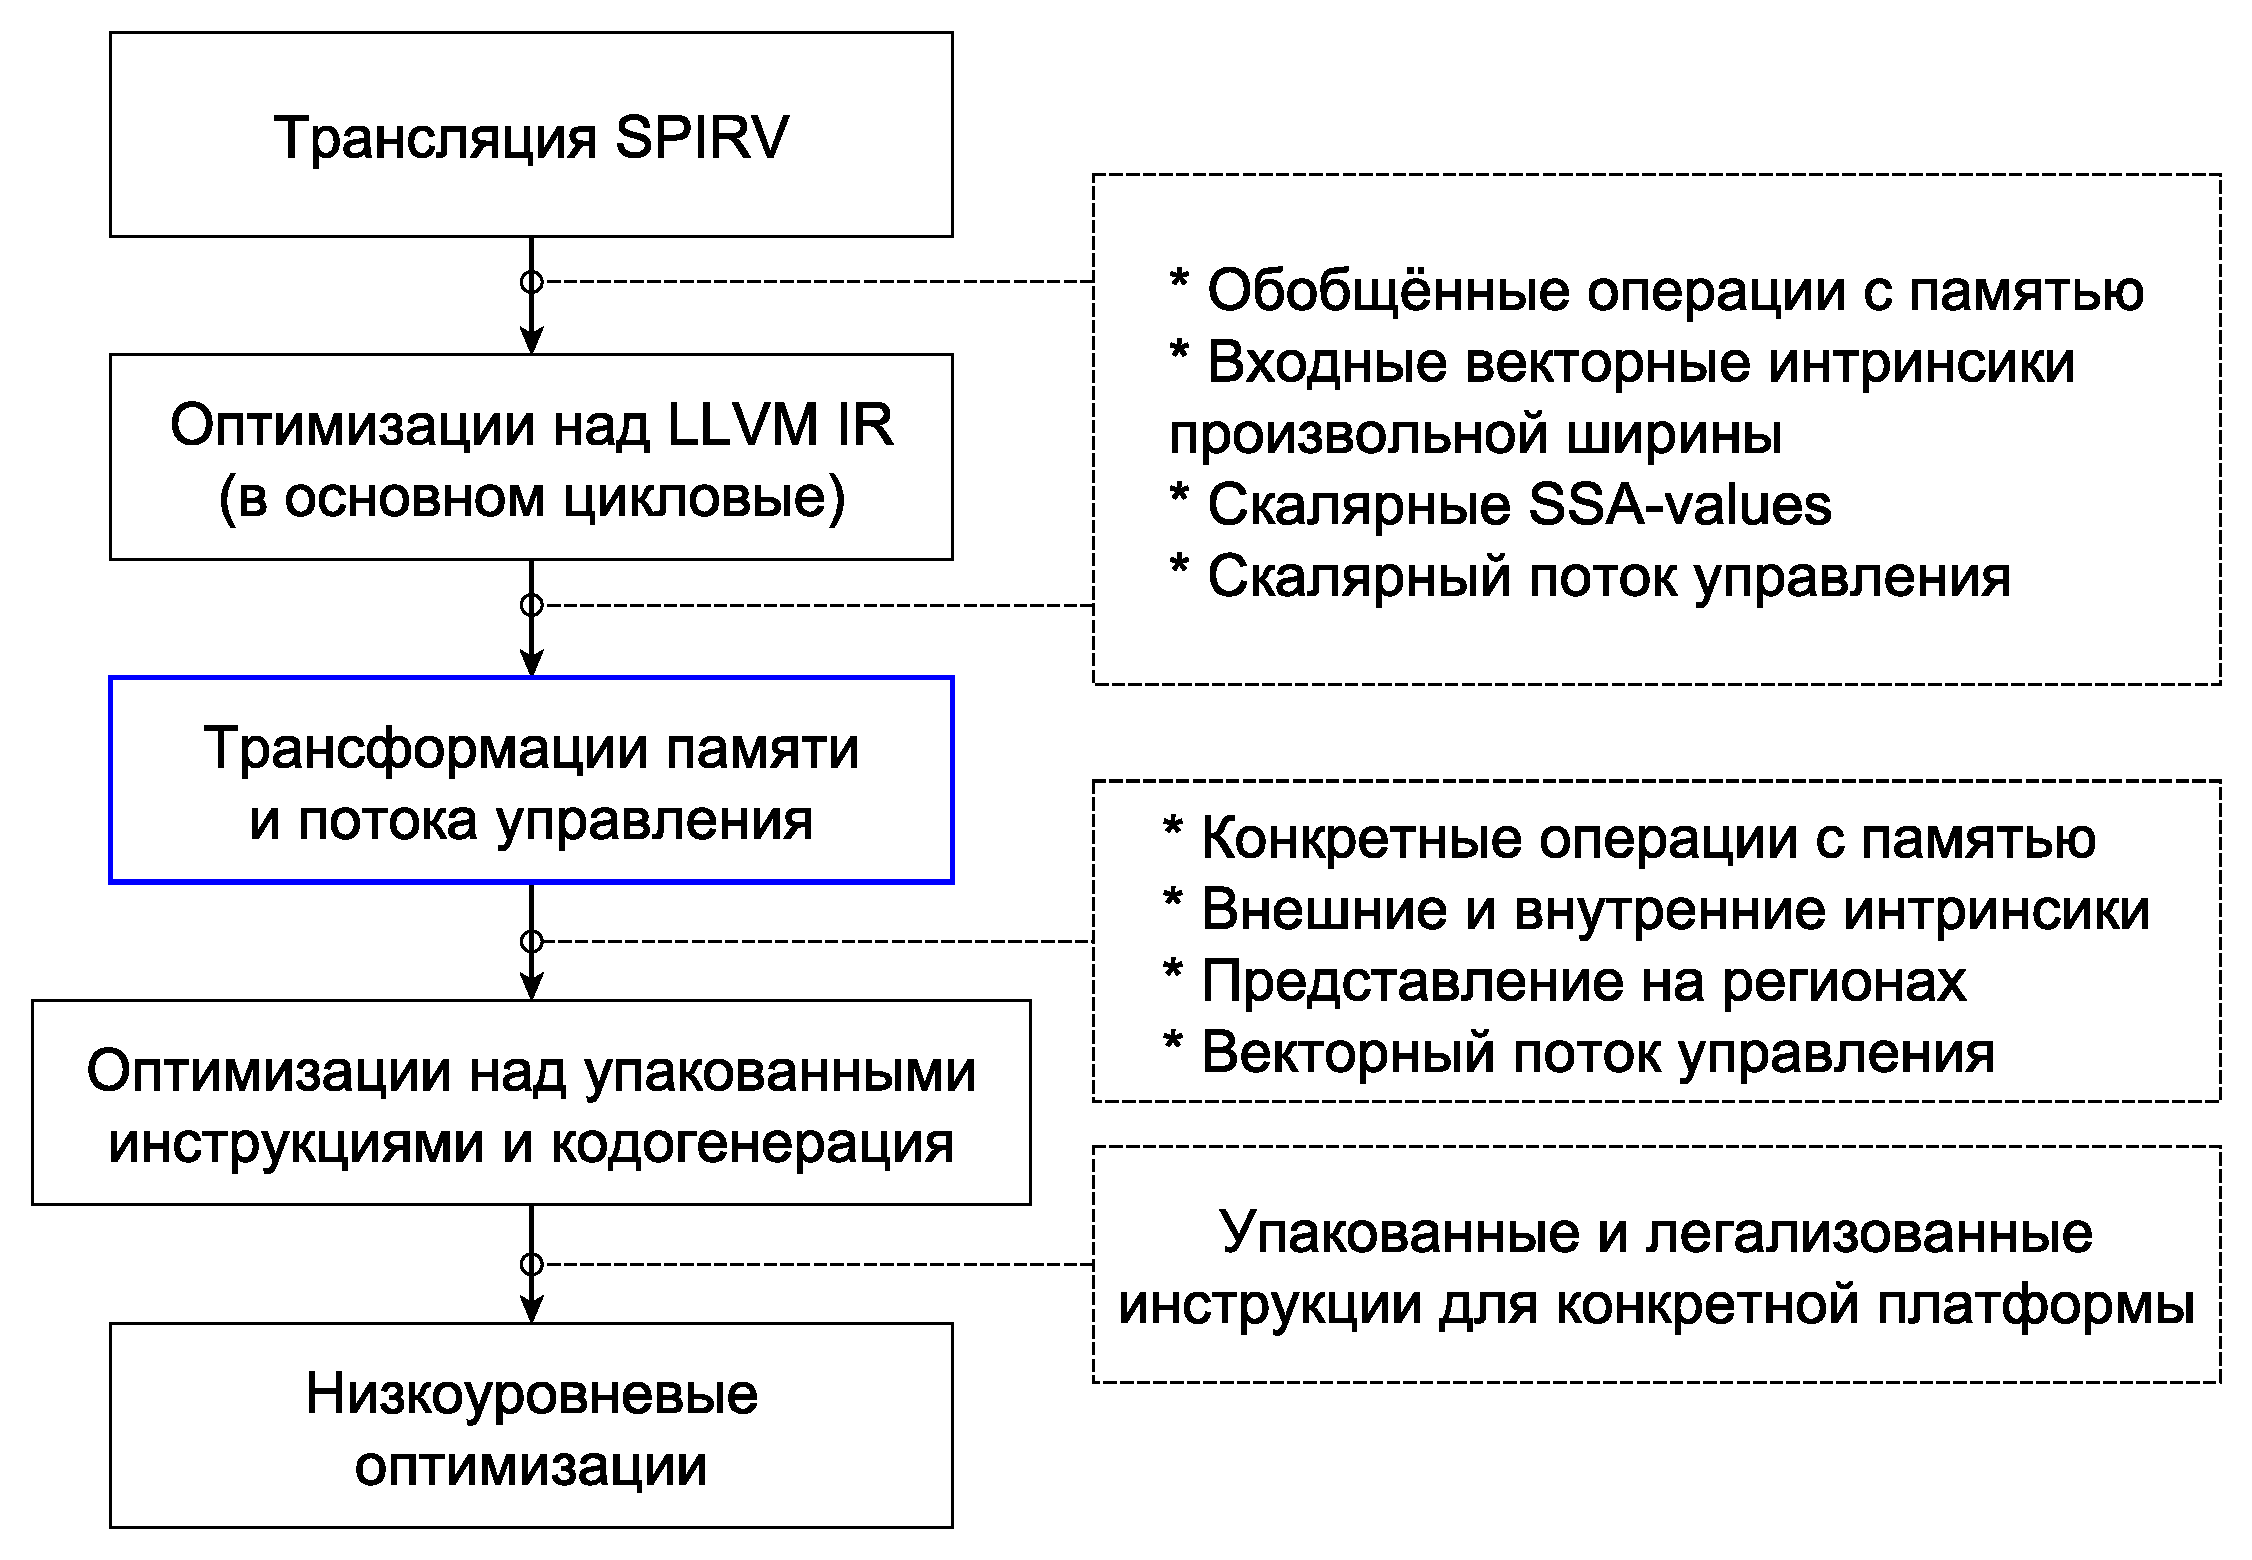
\includegraphics[scale=0.4]{Vladimirov/images/highlevel-mgr-inv.pdf}
    }
    \caption{Инварианты при трансформациях}\label{fig:highlevel-mgr-inv}
\end{figure}

После оптимизаций над высокоуровневым представлением, память не обязательно представляется исключительно обобщёнными операциями. Например программист может написать явный векторный код, работающий с векторными загрузками из памяти. В этом случае высокоуровневые оптимизации вряд ли будут способны обработать такую операцию и на вход каскадного понижения она попадёт в неизменном виде.

\subsection{Представление на регионах}\label{subsec:lowering/passes/lowlevel}

Физическое представление на регионах может существовать во многих формах. Например в графическом компиляторе Intel оно существует в виде G4IR, в виде VISA и в виде XeISA. 

\begin{ListingEnv}[!h]
    \captiondelim{ } 
    \caption{Пример физического представления}\label{lst:lowering/regrep}
    \begin{Verb}
mov (1|M0) r5.0<1>:uq r2.2<0;1,0>:uq
send (8|M0) r1 r5 0xC 0x021D0AFF
mov (1|M0) r6.0<1>:uq r2.3<0;1,0>:uq
send (8|M0) r3 r6 0xC 0x021D0AFF
add (8|M0) r4.0<1>:f r1.0<8;8,1>:f r3.0<8;8,1>:f
mov (1|M0) r7.0<1>:uq r2.1<0;1,0>:uq
sends (8|M0) r7 r4 0x4C 0x020D42FF
    \end{Verb}
\end{ListingEnv}

Листинг~\cref{lst:lowering/regrep} показывает типичное представление на регионах того же самого кода, который высокоуровнево представлен на листинге~\cref{lst:lowering/irrep}.

Каждый регион соответствует обращению в регистровый файл GPU, тогда как функции send (называемые также внешними функциями) отвечают за общение с памятью, являясь максимально низкоуровневыми и специфичными для конкретной видеокарты.

Ниже будут рассмотрены две важные оптимизации, происходящие на пути снижения промежуточного представления от высокоуровневых операций с памятью до регионов и использования внешних функций.

\section{Разбиение структур}\label{sec:lowering/splitter}

\subsection{Выделение частей агрегатных типов для векторизации}\label{subsec:lowering/splitter/vectorization}

Перед описанием алгоритма разбиения определим правила, по которым мы будем выделять части агрегатных типов для векторизации.

В стандарте C++ существует концепция скалярного типа. Скалярными называются арифметические типы, типы перечислений, указатели и cv-квалифицрованные версии перечисленных типов. Назовём \emph{базовым} скалярный тип, поддерживаемый данной оптимизацией. В это множество входят также векторные типы, которых нет в C++, но которые есть в LLVM IR.  В это множество не входят, например, указатели. Определение сознательно является несколько нечетким, чтобы заложить возможность будущего расширения. Алгоритм ниже не разбивает базовые типы.

Назовём \emph{примитивным} либо базовый тип, либо агрегатный тип, у которого типы всех элементов одинаковы и примитивны. Такой тип нет необходимости делить, так как объекты таких типов могут быть легко переделаны в вектора фазой aggregate lowering, которая представлена в векторном оптимизаторе IGC. Для алгоритма нет разницы между примитивным типом и базовым, из которого этот примитивный тип состоит, поэтому примитивный всегда будет сводиться к базовому. Например, \verb|< 3 x [ 5 x int]>| будет эквивалентен типу \verb|int|.

Целью алгоритма разбиения структур является приведение всех структур в модуле (например в модуле LLVM IR) к структурам примитивного типа с обязательным сохранением поведения исходной программы в рамках as-if rule.

Фаза разбиения структур в векторном компиляторе разрабатывалась специально для ISPC -- компилятора для SPMD~(single program, multiple data). При этом алгоритм сам по себе может быть использован в более широких классах оптимизаторов, даже не основанных на LLVM. Оптимизация работает над LLVM модулем и должна применятся до векторизации.

Разбиение невозможно, если:
\begin{enumerate}
\item элемент структуры является указателем на другую нетривиальную структуру, в том числе на саму себя.
\item на структуру взят указатель.
\end{enumerate}

Первое ограничение появляется из-за использования версии LLVM, в которой ещё не были введены opaque указатели.
Собственноручная поддержка таких указателей приводит к сильному разрастанию получаемого модуля и невозможности применения других оптимизаций.
По этой же причине была невозможна поддержка передачи структур в пользовательские функции.
Второе ограничение связано с тем, что замена кода работы с указателем на аналогичный код с поделёнными структурами может привести к значительному увеличению количества инструкций.

Алгоритм был опубликован в \cite{vladimirov2022opt2}.

\subsection{Описание алгоритма}\label{subsec:lowering/splitter/algorithm}

\textbf{Шаг 1. Сбор информации о структурах в модуле}\\

Информация о структуре хранится в виде хэш-таблицы, где ключ -- это примитивный тип элемента, а значения -- элементы, соответствующие этому типу. Структура в дальнейшем будет делиться как раз по элементам этой хэш-таблицы, так как ключам будет соответствовать примитивный тип, а значениям -- элементы будущей структуры. 
Количество ключей минус один -- столько структур необходимо будет сгенерировать.
Соответственно, если у структуры существует только один примитивный тип, то данную структуру делить нет необходимости, так как она сама является примитивной.\\

\textbf{Шаг 2. Построение графа вложенности структур}\\

Граф строится следующим образом: вершине $A$ соответствует структура \%A. Ребро от вершины $C$ в вершину $A$ проводится в том случае, если структура, соответствующая вершине $A$, вложена в структуру, соответствующую вершине $C$. Назовём узлом-источником($Head$) вершину, которая соответствует типу, не вложенному ни в какие другие типы. Узлов-источников может быть как один, так и несколько, но не более одного. Такой способ построения позволяет разрешать случаи, когда один структурный тип вложен в несколько других структурных типов и в него в свою очередь вложено несколько базовых типов. Эффективное разделение на базовые типы в пригодном для векторизации ключе также делает возможными другие оптимизации.

\begin{figure}[ht]
    \centerfloat{
        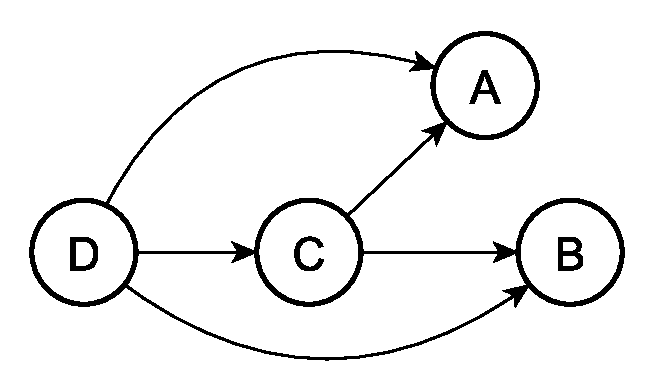
\includegraphics[scale=0.7]{Vladimirov/images/struct-orig.pdf}
    }
    \caption{Граф вложенности структур}\label{fig:struct-orig}
\end{figure}

\begin{ListingEnv}[!h]
    \captiondelim{ } 
    \caption{Пример структур для разбиения}\label{lst:lowering/struct-orig}
    \begin{lstlisting}[language={[ISO]C++}]
struct A { f32, <5 x f32> };
struct B { i32, <5 x i32> };
struct C { A, B };
struct D { A, i32, B, C};
    \end{lstlisting}
\end{ListingEnv}

Типичная структура для разбиения приведена на рисунке~\cref{fig:struct-orig} и описана в листинге~\cref{lst:lowering/struct-orig}.\\

\textbf{Шаг 3. Обработка графа вложенности структур}\\

Обработка графа начинается с узла источника, а процесс разбиения -- с самой нижней вершины. Все нижние вершины всегда характеризуются тем, что структуры, связанные с ними содержат элементы только примитивных типов, а значит данные структуры могут быть разбиты далее. При обработке вершины графа возможны два варианта.
Первое -- если вершина отвечает за примитивную структуру, то в разбиении нет необходимости и данная вершина удаляется из графа.
Второе -- структура, отвечающая за вершину была разбита на части. Тогда нужно заменить во всех структурах, в которые была вложена данная, все элементы, отвечающие за данную структуру, на новые элементы с учётом разбиения.
Во время замены элементов появляются промежуточные представления структур, которые затем необходимо удалить.
После обработки вершины она удаляется, поэтому все структуры будут обработаны тогда, когда весь граф будет свёрнут до единичной вершины.

\begin{figure}[ht]
    \centerfloat{
        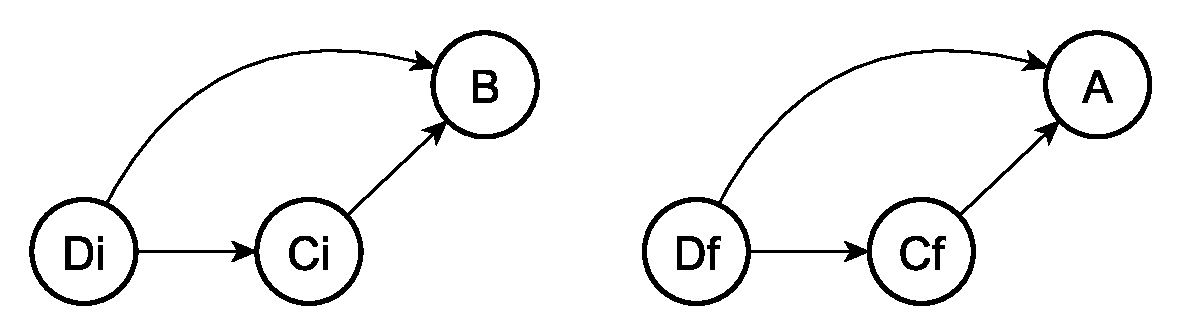
\includegraphics[scale=0.8]{Vladimirov/images/struct-splitted.pdf}
    }
    \caption{Разбитые структуры}\label{fig:struct-splitted}
\end{figure}

На рисунке~\cref{fig:struct-splitted} проиллюстрировано итоговое разбиение структуры, изображённой на рисунке~\cref{fig:struct-orig}.
Видно что структурные типы перегруппированы по входящим в них базовым типов, что и завершает разбиение.

Последняя проблема которую далее надо решить это замена всех инструкций которые работали с обрабатываемым типом так как после разбиения они очевидно будут работать с теми же участками памяти в другом порядке.

\textbf{Шаг 4. Обработка и замена инструкций}\\

Этот шаг зависит от конкретной реализации и будет разным в случае использования разного промежуточного представления. Мы подробно обсудим его позднее в разделе~\cref{subsec:results/igc/splitted}.

\section{Восстановление векторного потока управления}\label{sec:lowering/simdcf}

\subsection{Интерфейс между языками высокого уровня и векторным компилятором}\label{sec:lowering/simdcf/intface}

Одним из языков, используемых для разработки программ исполняемых на видеокартах, является ISPC \cite{pharr2012ispc}. ISPC (Implicit SPMD Program Compiler) -- язык программирования, являющийся расширением С и реализующий концепцию SPMD (single program, multiple data). ISPC является языком с раздельным исходным кодом. Изначально целевой архитектурой для данного языка была только архитектура x86 с векторными расширениями, но позже была добавлена поддержка для ARM процессоров с расширениями Neon, а также графических ускорителей Intel XE. Этот язык был подробно описан в разделе~\cref{subsec:overview/vectorapi/ispc}.

Программа на языке ISPC является SPMD программой и компилируется для векторов заранее известной зафиксированной длины. В такой программе могут обрабатываться как общие для всех потоков данные, так и свои данные для каждого запущенного потока. Общие данные отмечают как uniform переменные (то есть не изменяющиеся в зависимости от векторной линии), остальные по умолчанию считаются varying (то есть изменяющиеся). Таким образом любую varying переменную можно рассматривать как элемент вектора.

На листинге~\cref{lst:lowering/spmd-func} приведен пример типичной SPMD функции.

\begin{ListingEnv}[!h]
    \captiondelim{ } 
    \caption{Пример структур для разбиения}\label{lst:lowering/spmd-func}
    \begin{lstlisting}[language={[ISO]C++}]
void simple(uniform float vin[],
            uniform float vout[],
            uniform int count) {
  foreach (index = 0 ... count) {
    float v = vin[index];
    if (v < 3.)
        v = v * v;
    else
        v = sqrt(v);
    vout[index] = v;
  }
}
    \end{lstlisting}
\end{ListingEnv}

В SPMD языках нет ограничений на векторный поток управления. В стандартных конструкциях языка он реализуется через использование в качестве условия varying переменной. При этом, так как такого рода языки часто бывают кроссплатформенными (и поддерживаемые ими архитектуры различаются действительно кардинально) использование платформенно-специфичных интринсиков нежелательно. Вместо этого они маскируют результаты операций после условных переходов для векторного потока управления. Для архитектуры графических ускорителей Intel такой подход не позволяет использовать всех векторных возможностей потока управления, предоставляемых аппаратурой.

В связи с этим предлагается интефейс для языков высокого использующих векторный backend графического компилятора Intel. Так как интерфейс должен представлять собой конструкцию на промежуточном представлении (например LLVM IR), который не поддерживает векторный поток управления, неизбежно возникает необходимость сводить векторное условие к скалярному виду. Перед условным переходом необходимо проверить справедливо ли условие хоть для одного элемента и выполнять переход только в таком случае. Для наибольшей кроссплатформенности для подобных проверок следует использовать стандартные интринсики LLVM \texttt{@llvm.vector.reduce.and} и \texttt{@llvm.vector.reduce.or}. Также для языков высокого уровня, поддерживающих только архитектуру графических ускорителей Intel как целевую (например CM), допускается использовать для редукции условий платформозависимые интринсики \text{@llvm.genx.any} и \text{@llvm.genx.any}, являющиеся полными аналогами прежде упомянутых. Для сохранения семантического смысла и поддержки платформ, на которых нет развитой поддержки векторного потока управления, необходимо маскировать условием побочные эффекты дуги перехода.

\begin{figure}[ht]
    \centerfloat{
        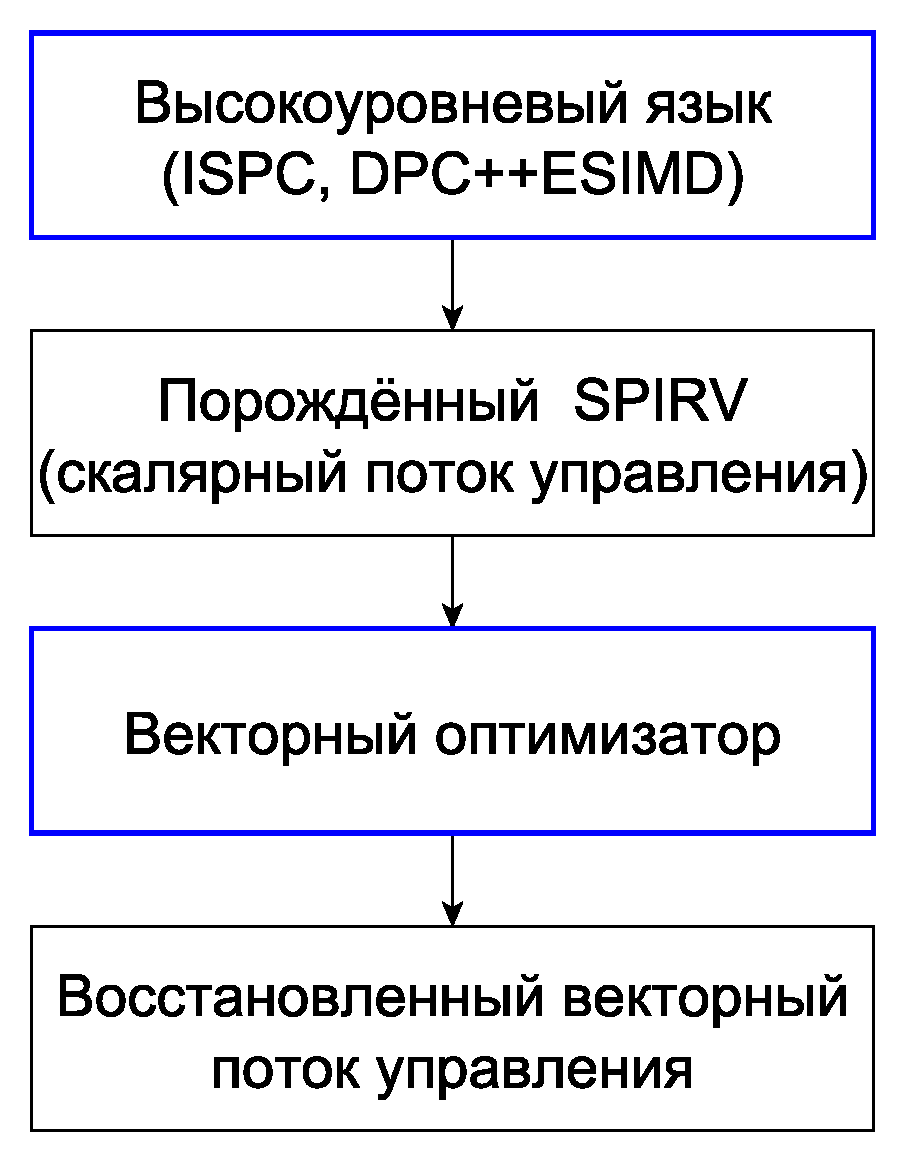
\includegraphics[scale=0.6]{Vladimirov/images/simdcf-gen.pdf}
    }
    \caption{Место восстановления SIMDCF в pass manager}\label{fig:simdcf-gen}
\end{figure}

Место такого рода восстановления в общем конвейере графических оптимизаций показано на рисунке~\cref{fig:simdcf-gen}.

Данный подход также применим для скалярных архитектур, поддерживающих необходимые минимальные векторные расширения. При этом в процессе оптимизаций компилятор не сможет сделать трансформации ломающие порядок побочных эффектов, поэтому такая конструкция будет валидна на всех этапах своего существования.

Существует обширная литература как по сопоставлению графов потока управления \cite{matoussi2019loop} так и по оптимизации для обобщённых flow graphs \cite{mansky2016specifying}.

\subsection{Поиск конструкций векторного потока управления}\label{sec:lowering/simdcf/optimization}

Алгоритм был опубликован в \cite{vladimirov2022opt}.

После определения SIMD CF региона можно свести задачу поиска заранее оговоренных конструкций к поиску SIMD CF регионов самого внешнего уровня вложенности, после чего искать вложенные SIMD CF регионы.\\

\textbf{Шаг 1.} Поиск условного перехода, похожего на векторный поток управления. Для каждого базового блока проверяется его терминатор. Если это инструкция условного перехода, то проверяется его условие, в противном случае конструкция не является SIMD CF регионом. Если условием является результат вызова одного из обозначенных ранее интринсиков, то идет переход к шагу 2.\\

\textbf{Шаг 2.} Проверяется структура потока управления и происходит попытка сопоставить его либо с SIMD CF if/else, либо с SIMD CF циклом. Если сопоставление с одним из заданных паттернов невозможно, то конструкция не является SIMD CF регионом. В противном случае происходит переход к шагу 3.\\

\textbf{Шаг 3.} Проверка маскирования побочных эффектов. Для каждой инструкции, у которой есть побочные эффекты проводится проверка, является ли такая инструкция маскирована и если она маскирована, то проверяется, совпадает ли маска для данной инструкции с условием перехода в эту дугу. Для вложенных регионов проверяется, является ли маска данного региона подмножеством маски внешнего региона. Если проверка неудачная - данный регион не является SIMD CF регионом.

Дополнение к шагу 3 для цикла. Проверяются фи-узлы для индуктивностей и пересчет маски для каждого цикла. Если проверка неудачная - данный регион не является SIMD CF регионом. В противном случае идет переход к шагу 4.

Дополнение к шагу 3 для if-else. Если кроме if также имеется else, то происходит проверка, являются ли маски if и else строго противоположны друг другу. Если проверка неудачная - данный регион не является SIMD CF регионом. В противном случае идет переход к шагу 4.\\

\textbf{Шаг 4.} Данный регион является SIMD CF регионом. Аналогично происходит поиск вложенных SIMD CF регионов для данного региона.

В псевдокоде данный алгоритм будет выглядеть как показано на листинге~\ref{lst:simdcf-analysis} который приведён в приложении.

\subsection{Трансформация конструкций векторного потока управления}\label{sec:lowering/simdcf/transform}

После сбора всей информации о SIMD CF регионах начинается их оптимизирующая трансформация.

\begin{figure}[ht]
    \centerfloat{
        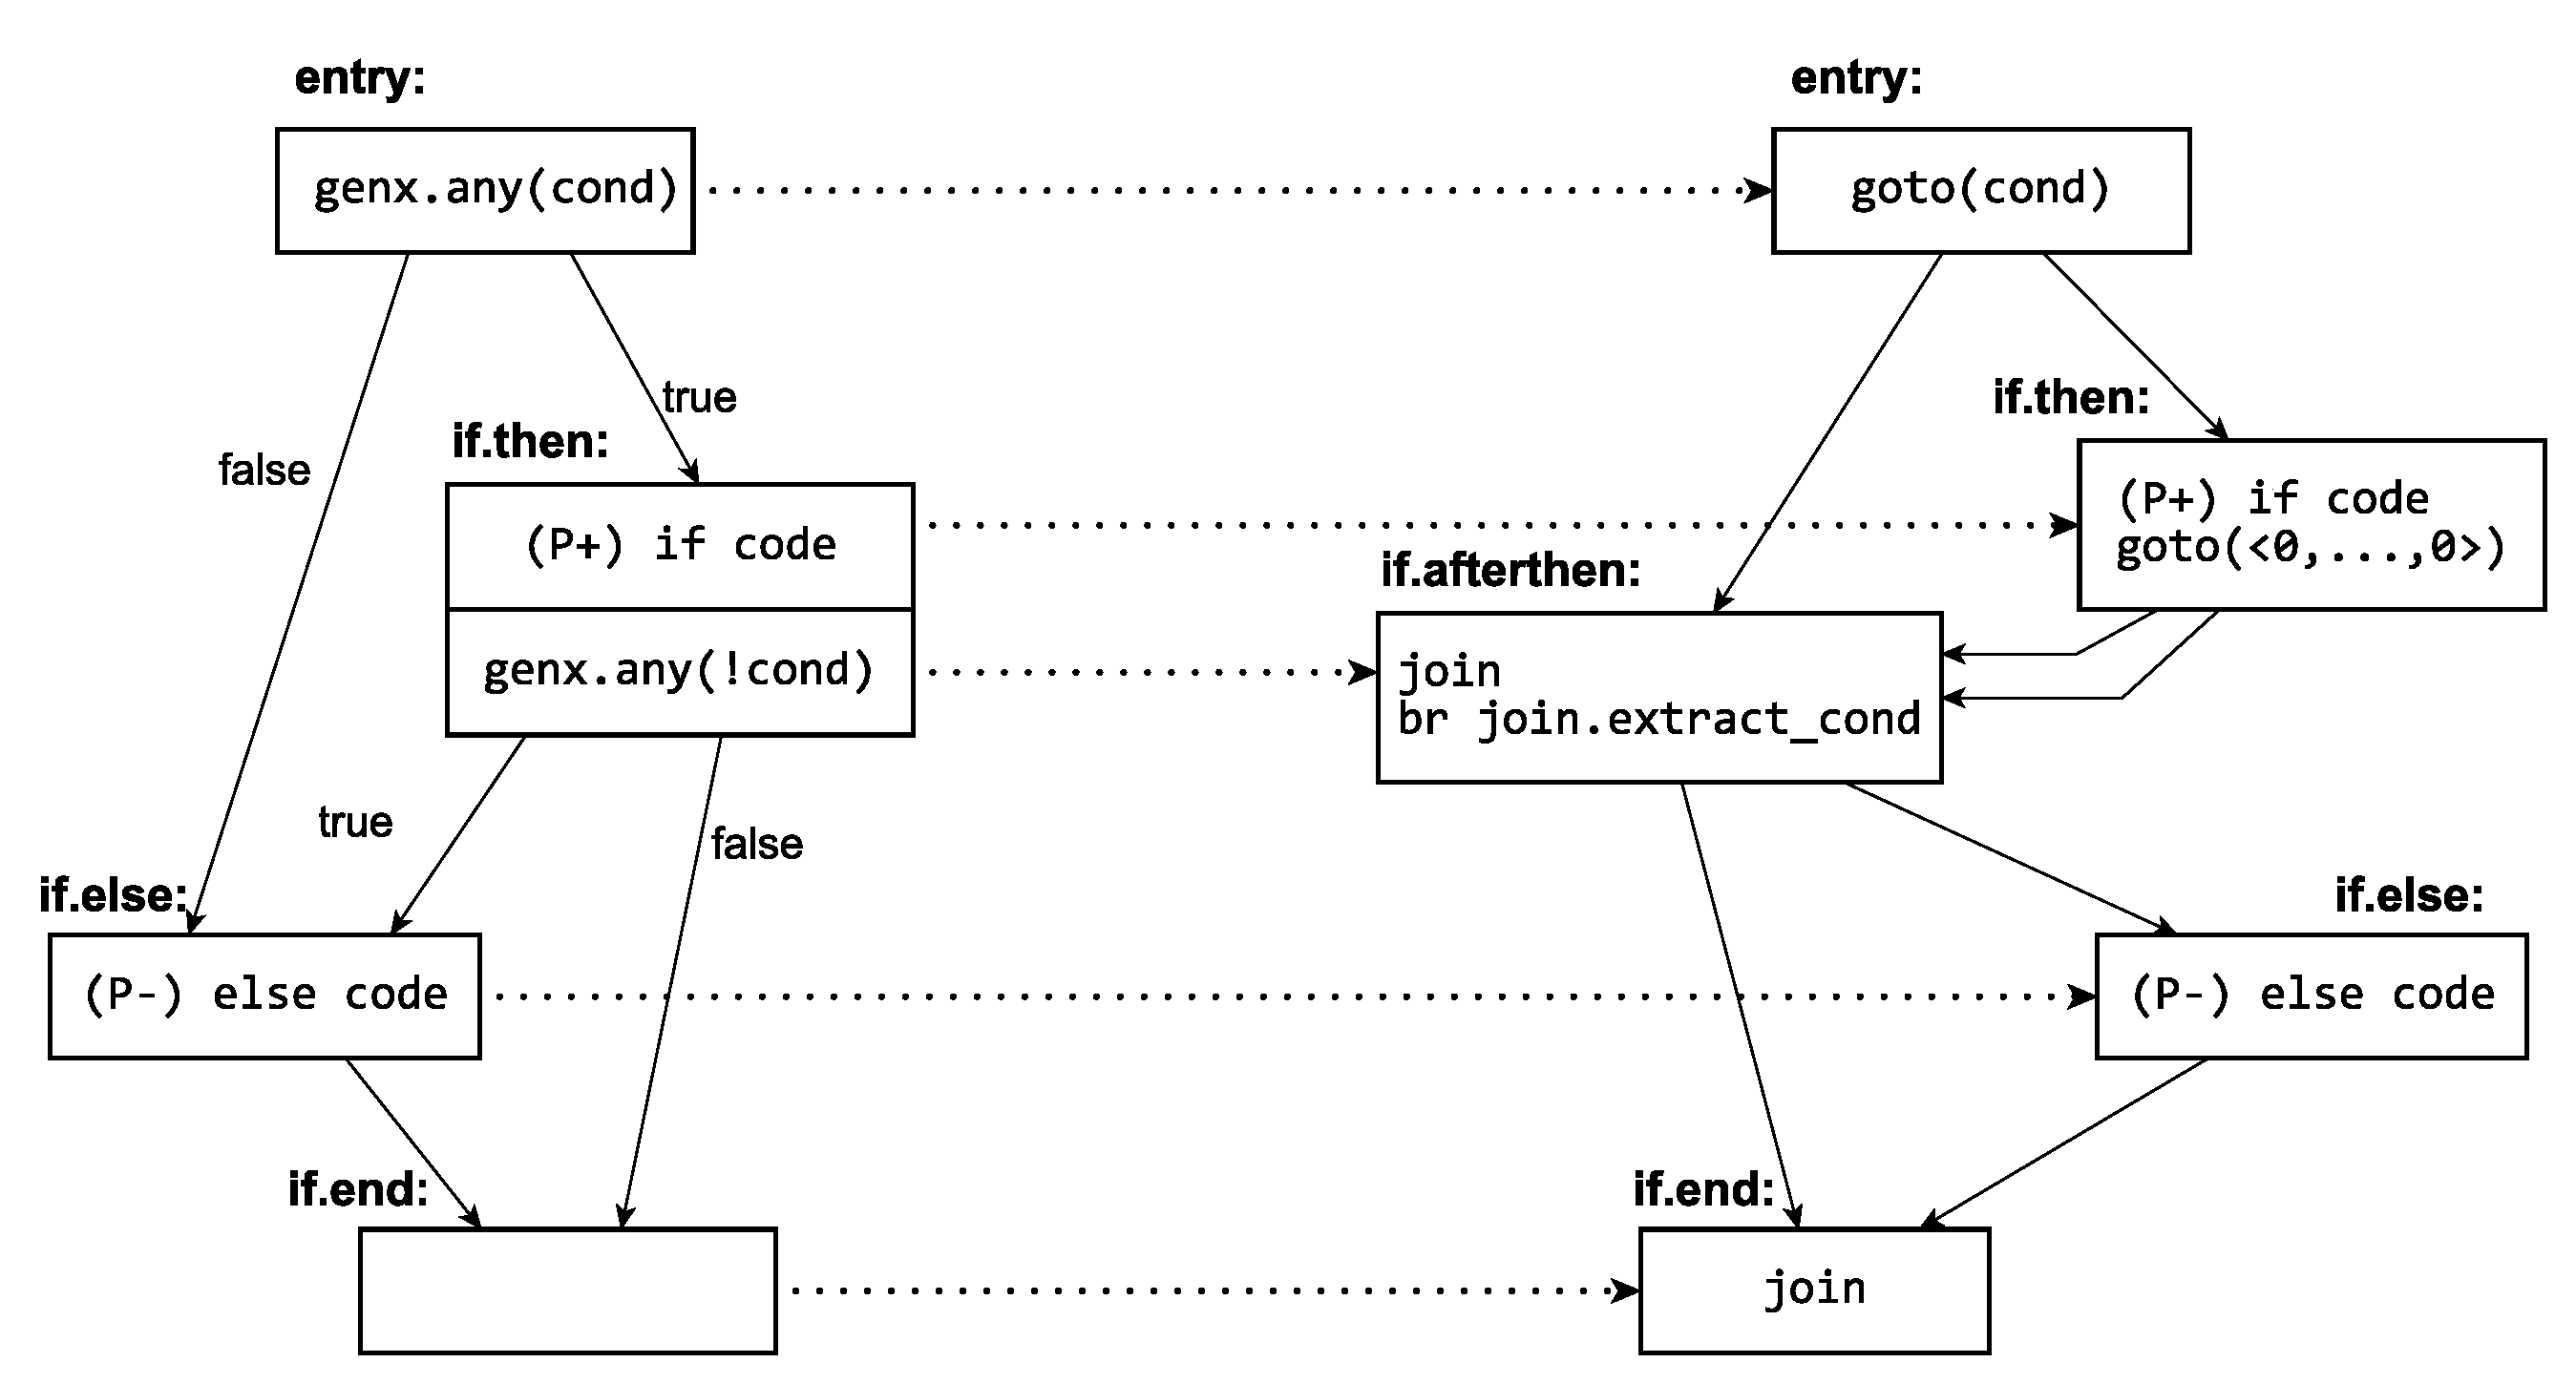
\includegraphics[scale=0.4]{Vladimirov/images/if-else-BE.pdf}
    }
    \caption{Восстановление if-else SIMD}\label{fig:if-else-BE}
\end{figure}

Пример трансформации условия приведён на рисунке~\ref{fig:if-else-BE}.

\section{Выводы}\label{sec:lowering/outcome}

Во второй главе описывается метод ступенчатого понижения промежуточного представления, алгоритм разбиения структур и алгоритм восстановления векторного потока управления.

При описании метода ступенчатого понижения, описываются его основные ограничения и допущения. Метод состоит из нескольких трансформаций, трансформации разбиты на функциональные и оптимизационные. Каждая трансформация подробно рассматривается, указывается её место в общей картине и взаимодействие с другими трансформациями. Описываются инварианты трансформаций, а также их входной и выходной формат: обобщённое высокоуровневое представление и представление на регионах.

При описании алгоритма восстановления векторного потока управления описывается интерфейс между языками высокого уровня и векторным компилятором, мотивируется почему этот интерфейс должен быть скалярным и предикатным. Далее описывается в общих чертах алгоритм восстановления векторного потока управления (детально он описан в прложении). После того как основные конструкции распознаны, описывается трансформация, восстанавливающая их в оптимизаторе.

При описании алгоритма разбиения структур описывается механизм выделения частей агрегатных типов для векторизации. Далее в деталях описывается сам алгоритм разбиения структур, включающий построение графа вложенности и нетривиальную обработку этого графа.

\FloatBarrier